\documentclass[thesis]{subfiles}

\begin{document}
	
	\chapter{Deep Roots}
	\label{deeproots}
	
	
	It is well understood that the structure of a neural network is critical to its ability to learn from labelled training data and to generalize. Whilst it has been shown that an infinitely wide hidden layer is a universal approximator~\citep{hornik89a}, in practice wide shallow networks do not learn as well as thinner deeper ones -- as shown by recent research~\citep{Krizhevsky2012imanet,Szegedy2014going,Simonyan2014verydeep,He2015}.
	This does not appear to be a limitation of finite capacity, since deep networks have been shown to be representable by shallow networks~\citep{Ba2013dothey}. Rather it seems to be a consequence of limitations in our methods of learning the weights of deep networks.
	
	It has been shown that a large proportion of the learned weights in deep networks are redundant~\citep{Denil2013predicting} (a property that many have attempted to exploit to make neural networks smaller and more computationally efficient~\cite{Szegedy2014going,Denton2014efficient}). It is unsurprising then that regularization is a critical part of training such networks using large training datasets~\cite{Krizhevsky2012imanet}. Without regularization (e.g. weight decay, dropout~\cite{1207.0580v1}) deep networks are susceptible to severe over-fitting (see \S\ref{regularization}). Aside from different training methods, a carefully designed network connection structure can have a regularizing effect in and of itself. Convolutional Neural Networks (CNNs)~\citep{Fuk80,Lecun1998} embody this idea, exploiting prior knowledge of the locality of natural image structure to design neural architectures with more limited, but salient, connectivity than a fully-connected neural network, that is in turn easier to learn. More recently, learning CNNs with low rank filters was found to have a regularizing effect, improving generalization compared to a CNN with only full rank filters~\citep{Ioannou2016}.
	
	With few exceptions, state-of-the-art CNNs for image recognition are largely monolithic -- convolutional neural networks with each filter operating on the feature maps of all filters on a previous layer, presenting no significant per-layer heterogeneity. Interestingly, this is in stark contrast to what we understand of biological neural networks, where we see ``highly evolved arrangements of smaller, specialized networks which are interconnected in very specific ways''~\citep{minsky1988perceptrons}.
	% Try to find a creative commons version of this
	%\begin{figure}[t]
	%\centering
	%\includegraphics[width=0.25\columnwidth, page=1]{figs/tree_root.jpg}
	%\caption{This work introduces the idea of using hierarchical filter grouping to create CNN connection structures that resemble tree roots. Applying the technique to existing state-of-the-art networks allows improved efficiency without compromising accuracy.}
	%\label{fig:tree}
	%\end{figure}
	
	% Maybe we need something like this here too, don't know
	%It has been shown that reducing the co-adaption of filters is beneficial to generalization in deep networks~\citep{1207.0580v1,goodfellow2013maxout,Cogswell2016}. Co-adaption occurs when hidden layer filters (or neurons) rely on one another to fit training data, such that their outputs become highly correlated. However, instead of using a modified loss, regularization penalty, or randomized network connectivity during training to prevent co-adaption of features, we take a much more direct approach. We use hierarchical filter groups (see \S\ref{regularizingstructure}) to allow the network itself to learn independent filters. By restricting the connectivity between filters on subsequent layers the network is forced to learn filters of limited dependence. We allow the standard network optimization (\eg SGD) to learn appropriate weights within this restricted architecture.
	
	In this paper we show that simple alterations to the architecture of state-of-the-art CNNs for image recognition can drastically reduce computational cost and model size while maintaining (or even increasing) accuracy, through structure-induced regularization, by reducing the connectivity in monolithic networks to reflect more closely the sparse, localized filter co-dependencies within.
	
	\section{Related Work}
	\label{previouswork}
	
	
	\subsubsection{Reducing Co-dependence in Deep Networks.}
	\label{regularization}
	\citet{1207.0580v1} introduced {\em dropout} for regularization of deep networks. When training a network layer with dropout, a random subset of neurons is excluded from both the forward and backward pass for each mini-batch. Effectively a different (random) network topology is trained at each iteration. As the authors observe, this approach has some similarities with that of using model ensembles, another effective way to increase generalization. However, one limitation of dropout is that it increases the number of training iterations required for convergence, typically by a factor of two. Recently, \citet{Szegedy2014going} have suggested that dropout provides little incremental accuracy improvement compared to simply training using {\em batch normalization}. 
	
	\citet{Cogswell2016} observe a correlation between the cross-covariance of hidden unit activations and overfitting. To explicitly reduce the cross-covariance of hidden activations, they train networks with a loss function, based on the covariance matrix of the activations in a hidden layer. \citet{Cogswell2016} use this loss on the fully connected layers at the end of deep networks such as AlexNet and demonstrate an increase in generalization accuracy comparable with that obtained by using dropout.
	
	%:
	%\begin{equation}
	%	C_{i,j} = \frac{1}{N} \sum^N_{n = 0} (h_i^n - \mu_i)(h_j^n - \mu_j),
	%	\label{eqn:covariance}
	%\end{equation}
	%where $n$ is a sample in a mini-batch of size $N$, $i$ and $j$ index a pair of activations within the mini-batch, and $\mu_i$ is the sample mean over the batch. The `DeCov' loss is defined as:
	
	%\begin{equation}
	%	L_{\textrm{\texttt{DeCov}}} = \frac{1}{2} \left( \|C\|^2_F - \|diag(C)\|^2_2 \right).
	%	\label{eqn:decov}
	%\end{equation}
	
	\subsubsection{Reducing Model Size and Computation.}
	\label{regularizingstructure}
	Most previous work on reducing computation in CNNs has focused on the spatial extents of the convolutional filters in the form of low-rank spatial filters~\citep{mamalet2012simplifying,journals/corr/JaderbergVZ14, journals/pami/SironiTRLF15, journals/corr/LebedevGROL14, Ioannou2016}, using frequency-based convolution~\cite{mathieu2013fast,rippel2015spectral}. More general methods for speeding up CNNs have used reduced precision numerics~\cite{1502.02551v1} or pre-trained model compression~\cite{Chen2015,Kim2016}. Here we explore methods that reduce the computational impact of the large number of filter channels within state-of-the art networks. In particular, methods to decrease the number of filters and thus output feature map channels while maintaining accuracy (\ie the depth of filters, $c$ in Fig.~\ref{fig:normalconv} rather than the spatial extents ($h, w$)\,).
	
	\begin{figure}[t]
		\centering
		\begin{subfigure}[b]{0.66\columnwidth}
			\includegraphics[width=\columnwidth, page=1]{groupfig}
			\caption{Convolution with $d$ filters of shape $h\times w\times c$.}
			\label{fig:normalconv}
		\end{subfigure}
		~
		\begin{subfigure}[b]{0.66\columnwidth}
			\includegraphics[width=\columnwidth, page=2]{groupfig}
			\caption{Convolution with $d$ filters in $g$ filter groups, of shape $h\times w\times c/g$.}
			\label{fig:groupedconv}
		\end{subfigure}
		\caption{\textbf{Filter Groups.} (a) Convolutional filters (yellow) typically have the same channel dimension $c$ as the input feature maps (gray) on which they operate. However, (b) with filter grouping, $g$ independent groups of $d/g$ filters operate on a fraction $c/g$ of the input feature map channels, reducing filter dimension from $h$$\times$$w$$\times$$c$ to $h$$\times$$w$$\times$$c/g$. This change does not affect the dimensions of the input and output feature maps but significantly reduces computational complexity and the number of model parameters.}
		\label{fig:groupconfig}
	\end{figure}
	
	\paragraph{AlexNet Filter Groups.} Amongst the seminal contributions made by \citet{Krizhevsky2012imanet}~is the use of `filter groups' in the convolutional layers of a CNN (see Fig. \ref{fig:groupconfig}). While the use of filter groups was necessitated by the practical consideration of sub-dividing the work of training a large network across multiple GPUs, the side effects are somewhat surprising. Specifically, the authors observe that independent filter groups learn a separation of responsibility (colour features vs. texture features) that is consistent over different random initializations. Also surprising, and not explicitly stated in~\citep{Krizhevsky2012imanet}, is the fact that the AlexNet network has approximately 57\% fewer connection weights than the corresponding network without filter groups (see Fig.~\ref{fig:alexnetplots}). This is due to the reduction in the input channel dimension of the grouped convolution filters.
	Surprisingly, despite the large difference in the number of parameters between the models, both architectures achieve comparable error on ILSVRC -- in fact the smaller grouped network gets $\approx1$\% lower top-5 validation error. This paper builds upon and extends these findings to state-of-the-art networks.
	
\begin{figure}[tb]
	\centering
	\pgfplotstableread[col sep=comma]{rootdata/alexnetma.csv}\datatable
	\pgfplotsset{major grid style={dotted,red}}
	
	\begin{tikzpicture}
	\begin{axis}[
	width=\columnwidth,
	height=0.25\columnwidth,
	axis x line=bottom,
	ylabel=Top-5 Val.\ Error,
	xlabel=Model Parameters (\# floats),
	axis lines=left,
	enlarge x limits=0.10,
	enlarge y limits=0.1,
	grid=major,
	%xmin=0,
	ytick={0.01,0.02,...,0.21},
	ymin=0.18,ymax=0.2,
	yticklabel={\pgfmathparse{\tick*100}\pgfmathprintnumber{\pgfmathresult}\%},style={
		/pgf/number format/fixed,
		/pgf/number format/precision=1
	},
	legend style={at={(0.98,0.98)}, anchor=north east, column sep=0.5em},
	legend columns=2,
	]
	\addplot[mark=*,mark options={fill=black},nodes near coords,only marks,
	point meta=explicit symbolic,
	%   x filter/.code={
	%       \ifnum\coordindex>2\def\pgfmathresult{}\fi
	%   },
	] table[meta=Network,x=Param.,y expr={1 - \thisrow{Top-5 Acc.} },]{\datatable};
	%\addplot[mark=square*,mark options={fill=blue},nodes near coords,only marks,
	%   point meta=explicit symbolic,
	%   x filter/.code={
	%       \ifnum\coordindex<3\def\pgfmathresult{}\fi
	%   },
	%] table[meta=Network,x=Param.,y expr={1 - \thisrow{Top-5 Acc.} },]{\datatable};
	%\legend{Standard AlexNet}%, Alternate Filter Grouping}
	\end{axis}
	\end{tikzpicture}
	\caption{\textbf{AlexNet Filter Groups.} Model Parameters \vs top-5 error for variants of the AlexNet model on ILSVRC image classification dataset. Models with moderate numbers of filter groups have far fewer parameters, yet surprisingly maintain comparable error.}
	\label{fig:alexnetplots}
\end{figure}

	
	\paragraph{Low-dimensional Embeddings.}
	\citet{Lin2014} proposed a method to reduce the dimensionality of convolutional feature maps. 
	%As illustrated in Fig.~\ref{fig:lowdim}
	By using relatively cheap `1$\times$1' convolutional layers (i.e. layers comprising $d$ filters of size $1\times 1 \times c$, where $d<c$), they learn to map feature maps into lower-dimensional spaces, \ie to new feature maps with fewer channels. Subsequent spatial filters operating on this lower dimensional input space require significantly less computation. This method is used in most state of the art networks for image classification to reduce computation~\citep{Szegedy2014going,He2015}. Our method is complementary to low-dimensional embeddings. 
	
	%\begin{figure}[t]
	%\centering
	%\includegraphics[width=0.5\columnwidth, page=3]{figs/groupfig}
	%\caption{\textbf{Low-dimensional Embeddings.} $d$ 1$\times$1$\times$c filters (yellow) learn a transformation from a $c$-dimensional input feature map on which they operate into a $d$-dimensional output feature map.}
	%\label{fig:lowdim}
	%\end{figure}
	
	\paragraph{Conditional Networks.} \citet{Ioannou2015} describe conditional networks, \ie deep networks trained from random initialization with a tree-like structure of convolutional filter groups. This tree-like structure reduces computation, but can also reduce accuracy. Our results show that with a different structure of sparsity, not only can we reduce computation further, but we can maintain if not increase accuracy.
	
	\paragraph{GoogLeNet.} In contrast to much other work, \citet{Szegedy2014going} propose a CNN architecture that is highly optimized for computational efficiency. GoogLeNet uses, as a basic building block, a mixture of low-dimensional embeddings~\citep{Lin2014} and heterogeneously sized spatial filters -- collectively an `inception' module. 
	
	There are two distinct forms of convolutional layers in the inception module, low-dimensional embeddings (1$\times$1) and spatial (3$\times$3, 5$\times $5). GoogLeNet keeps large, expensive spatial convolutions (\ie 5$\times$5) to a minimum by using few of these filters, using more 3$\times$3 convolutions, and even more 1$\times$1 filters again. The motivation is that most of the convolutional filters respond to localized patterns in a small receptive field, with few requiring a larger receptive field. The number of filters in each successive inception unit increase slowly with decreasing feature map size, in order to maintain computational performance.
	
	GoogLeNet is by far the most efficient state-of-the-art network for ILSVRC, achieving near state-of-the-art accuracy with the lowest computation/model size. However, we will show that even such an efficient and optimized network architecture benefits from our method.
	
	\paragraph{Low-Rank Approximations.}
	Various authors have suggested approximating learned convolutional filters using tensor decomposition~\citep{journals/corr/JaderbergVZ14,journals/corr/LebedevGROL14,Kim2016}. For example, \citet{journals/corr/JaderbergVZ14} propose approximating the convolutional filters in a pre-trained network with representations that are low-rank both in the spatial and the channel domains. This approach significantly decreases computational complexity, albeit at the expense of a small amount of accuracy. By contrast, here we will show that by training our network from scratch with a sparse structure of filter connectivity, we can similarly decrease computation without having to train a larger network beforehand, or to perform an expensive post-processing step. Because we are not approximating existing weights, but allowing standard stochastic gradient descent (SGD) to optimize our network, we can even increase accuracy through increased regularization.
	
	\section{Hierarchical Filter Groups}
	\label{method}
	In this section we present the main contribution of our work -- an exploration of the use of hierarchical filter groups to decrease computational complexity and model size compared to state-of-the-art deep networks for image recognition.
	
	\subsection{Reduced Co-adaption and Filter Groups}
	It has been shown that reducing the co-adaption of filters is beneficial to generalization in deep networks~\citep{1207.0580v1,goodfellow2013maxout,Cogswell2016}. Co-adaption occurs when hidden layer filters (or neurons) rely on one-another to fit training data, becoming highly correlated. However, instead of using a modified loss, regularization penalty, or randomized network connectivity during training to prevent co-adaption of features, we take a much more direct approach. We use hierarchical filter groups (see \S\ref{regularizingstructure}) to allow the network itself to learn independent filters. By restricting the connectivity between filters on subsequent layers the network is forced to learn filters of limited interdependence.
	
	This reduced connectivity also reduces computational complexity and model size. Unlike methods for increasing the efficiency of deep networks by approximating pre-trained existing networks (see \S\ref{previouswork}), our models are trained from random initialization using stochastic gradient descent. This means that our method can also speed up training and, since we are not merely approximating an existing models' weights, the accuracy of an existing model is not an upper bound on accuracy of the modified model.
	
	\subsection{Network Topology}
	An exhaustive exploration of the possible topologies for filter grouping within state-of-the-art deep networks is prohibitively expensive. Instead we based our exploration on a restricted, but interesting, subset of hierarchical topologies, each of which is illustrated in Fig.~\ref{fig:networktopology}. 
	Each of these topologies makes different fundamental assumptions on the co-dependence of filters within each layer and overall network architecture.
	
	\begin{figure}[t]
		\centering
		\begin{subfigure}[b]{0.85\columnwidth}
			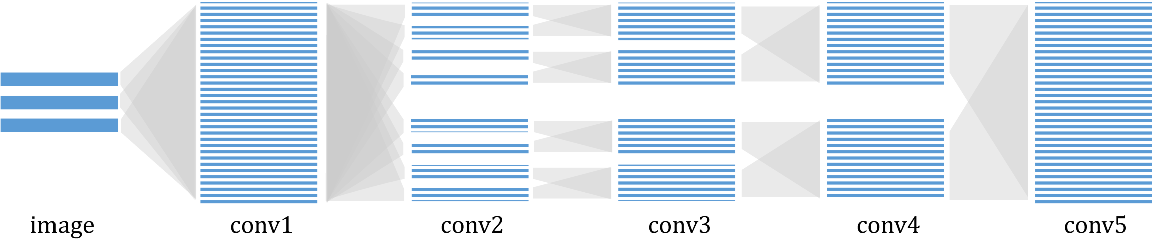
\includegraphics[width=\columnwidth, page=1]{networktopology}
			\caption{Root-8 topology}
			\label{fig:roottopology}
		\end{subfigure}
		~
		\begin{subfigure}[b]{0.85\columnwidth}
			\includegraphics[width=\columnwidth, page=2]{networktopology}
			\caption{Tree-2 topology}
			\label{fig:treetopology}
		\end{subfigure}
		~
		\begin{subfigure}[b]{0.85\columnwidth}
			\includegraphics[width=\columnwidth, page=3]{networktopology}
			\caption{Columnar-4 topology}
			\label{fig:columntopology}
		\end{subfigure}
		\caption{\textbf{Filter Group Network Topologies.} Topologies of filter groups explored, as illustrated in a VGG-style deep network. Grey blocks represent the input range over which a layer's filters operate, while coloured blocks represent the stacked feature maps of the filter groups within each layer. 
			%Root topologies assume that filters become more correlated with depth, while tree topologies assume filters become less correlated with depth.
		}
		\label{fig:networktopology}
	\end{figure}
	
	\subsubsection{Columns.} Columnar topologies assume that filters are consistently co-dependent with depth, and that this co-dependence is relatively small throughout the whole network. AlexNet uses a 2-column architecture on most layers.
	
	\subsubsection{Trees.} Tree-like topologies, as used by~\citet{Ioannou2016},  in conditional networks, assume that either filters become less co-dependent with depth, or the number of filters grows with depth enough that there are many more filters in deep layers than required. Notably,~\citet{Ioannou2016} evaluated their architecture on VGG networks, which are very large, and over-parametrized even compared to state-of-the-art networks such as residual networks.
	
	\subsubsection{Roots.} Root-like topologies (\ie inverted trees) assume that filters become more co-dependent with depth.  This aligns with the intuition of deep networks for image recognition subsuming the deformable parts model (DPM). If we assume that filter responses identify parts (or more elemental features), then there should be more filter co-dependence with depth, as more complex relationships emerge~\cite{girshick2015deformable}.
	
	In general, state-of-the-art CNN architectures have few filters in early convolutional layers, increasing throughout the network, and so it might seem that trees would have the best computational savings. Even so, the first few layers of a CNN are always the most computationally expensive, simply because the input feature map's spatial size is largest before any sub-sampling, in the layers close to the input image. As such, root topologies in general have the largest computational savings.
	
	%\subsection{Layer-wise Filter Covariance in Deep Networks}
	%We used the DeCov loss (see Eqn.~\ref{eqn:decov}) as a measure of the covariance of the filters on each convolutional layer. Although \citet{Cogswell2016} only use DeCov on fully-connected layers, we expanded it's use to convolutional layers by calculating the covariance of the average activation over each filter's feature map in a convolutional layer, rather than the activation of each neuron in a fully-connected layer. Instead of calculating batch statistics, the covariance and mean were calculated over a large random sample of training data.
	%\input{decovplot.tex}
	
	%\textit{Network in Network.}
	%For the NiN network, the DeCov loss was calculated over the entire CIFAR10 training set for a number of different model states from different training epochs, plotted on a log scale in Fig.~\ref{fig:decovplot_nincifar}. Even after a few training epochs the co-variance of filters in the first few layers is significantly reduced. The final network, after 300 epochs, shows a clear increase in co-variance with network depth, with layers close to the output layer having much higher covariance.
	
	%\textit{ResNet 50.}
	%Fig.~\ref{fig:decovplot} shows the per-layer DeCov loss for ResNet 50 plotted on a log scale. It was calculated over a 10000 random sub-sample of the ILSVRC training data for various training epochs. Clearly, filter covariance increases drastically with filter depth.
	
	%\textit{GoogLeNet.}
	%Fig.~\ref{fig:decovplot_googlenet} shows the per-layer DeCov loss for GoogLeNet plotted on a log scale, calculated over a 10000 random sub-sample of the ILSVRC training data. GoogLeNet is unusual in training with multiple intermediate losses. While each of the classifiers and fully-connected layers associated with the losses has high filter covariance, but the covariance of the composite responses of each of the inception units is relatively constant with depth, with the notable exception of `inception-4d'.
	
	%Given the results of our analysis of the layer-wise filter covariance in deep networks, we found filter covariance in deep networks be maintained or increase with depth. However, given that the number of filters per-layer increases rapidly with depth in all of these networks, on a per-filter basis, covariance is increasing. Given this, a root topology fits these findings best. 
	
	\section{Results}
	%Our approach is to explicitly separate convolutions within a network into many individual filter groups, similar to the approach of \citet{Ioannou2016}. However, instead of a tree-like topology, we propose that filters responses become more co-dependent with depth rather than less, and so a root-like topology is more appropriate.
	Here we present results of training from scratch re-structured (as described in \S\ref{method}) state-of-the-art network architectures for image classification on the CIFAR-10~\cite{CIFAR10} and ILSVRC~\citep{ILSVRC2015} datasets.
	
	\subsection{Improving Network in Network on CIFAR-10}
	Network in Network (NiN)~\cite{Lin2014} is a near state-of-the-art network for CIFAR-10~\cite{CIFAR10}. It is composed of 3 spatial (5$\times$5, 3$\times$3) convolutional layers with a large number of filters (192), interspersed with low-dimensional embedding (1$\times$1) layers. We replicated the standard NiN network architecture as described by \citet{Lin2014}, but with state-of-the-art training methods. We trained using random 32$\times$32 cropped and mirrored images from 4-pixel zero-padded  mean-subtracted images, as in~\citep{goodfellow2013maxout, He2015}. We also used the initialization of \citet{He2015delving} and batch normalization~\citep{Ioffe2015}. With this configuration, ZCA whitening was not required to reproduce validation accuracies obtained in~\citep{Lin2014}. We also did not use dropout, having found it to have little effect, presumably due to our use of batch normalization.

	\begin{table}[tbp]
		\caption[Network-in-Network CIFAR10]{\textbf{Network-in-Network CIFAR10}}
		\label{table:nincifarresults}
		\centering
		%\resizebox{\columnwidth}{!}{
		\pgfplotstableread[col sep=comma]{rootdata/nincifarbest.csv}\data
		
		\pgfplotstabletypeset[
		every head row/.style={
			before row=\toprule,after row=\midrule},
		every last row/.style={
			after row=\bottomrule},
		every first row/.style={
			after row=\bottomrule}, 
		fixed zerofill,     % Fill numbers with zeros
		columns={name, ma, param, accuracy, cpu, gpu},
		columns/name/.style={
			column name=Model,
			string type
		},
		columns/ma/.style={
			column name=FLOPS {\small $\times 10^{8}$},
			preproc/expr={{##1/1e8}}
		},
		columns/param/.style={
			column name=Param. {\small $\times 10^{5}$},
			preproc/expr={{##1/1e5}}
		},
		column type/.add={lrrrrrr}{},
		columns/accuracy/.style={
			column name=Accuracy,
			precision=4
		},
		columns/gpu/.style={
			column name=GPU (ms),
			precision=3
		},
		columns/cpu/.style={
			column name=CPU (ms),
			precision=1
		},
		highlight col max ={\data}{accuracy},
		highlight col min ={\data}{param}, 
		highlight col min ={\data}{ma}, 
		col sep=comma]{\data}
		%}
	\end{table}
	
	We restructured the network with hierarchical groups, while preserving the original number of filters per layer. To determine which of the network topologies in Fig.~\ref{fig:networktopology} gave the best computational savings with the minimal loss in accuracy, we implemented each for various numbers of initial filter groups.
	
	We only group filters within the the spatial (\ie non 1$\times$1) layers. Using filter groups within the low-dimensional embedding layers (\ie 1$\times$1 convolutions) leads to learning even lower dimensional embeddings of the input space, which is likely to compromise their representational ability. Indeed, in such configurations we observed a large decrease in accuracy. We also do not group filters in the first convolutional layer -- since it operates on the three-channel image space, it is of limited computational impact compared to other layers, and we believe learning color filters to be critical to learning. 
	
	Table~\ref{table:nincifarresults} lists the best results for each of the topologies.
	% (also plotted in Fig.~\ref{fig:nincifarplotsconvonly}).
	Only the root-like topology maintains accuracy while decreasing computation and model size significantly -- the best, root-4, has only 55\% of the floating point operations (FLOPS), 47\% of the model parameters of the original network, and approximately 22\% faster CPU and GPU timings.
	
	\begin{figure}[tbp]
		\centering
		\begin{subfigure}[b]{0.48\columnwidth}
			\pgfplotstableread[col sep=comma]{rootdata/nincifar.csv}\datatable
			\pgfplotstableread[col sep=comma]{rootdata/nincifar_root_s.csv}\rdatatable
			%\pgfplotstableread[col sep=comma]{rootdata/nincifar_col_s.csv}\cdatatable
			\pgfplotstableread[col sep=comma]{rootdata/nincifar_tree_s.csv}\tdatatable
			\pgfplotsset{major grid style={dotted,red}}
			
			\centering
			\begin{tikzpicture}
			tikzstyle{every node}=[font=\scriptsize]
			\begin{axis}[
			width=\columnwidth,
			height=0.66\columnwidth,
			axis x line=bottom,
			ylabel=Error,
			xlabel=Model Parameters,
			axis lines=left,
			enlarge x limits=0.05,
			enlarge y limits=0.2,
			grid=major,
			%xmin=0,
			%ytick={0.01,0.02,...,0.2},
			%ymin=0.075,ymax=0.09,
			xticklabel style={
				/pgf/number format/fixed,
				/pgf/number format/precision=3
			},
			yticklabel={\pgfmathparse{\tick*1}\pgfmathprintnumber{\pgfmathresult}\%},style={
				/pgf/number format/fixed,
				/pgf/number format/precision=1
			},
			]
			\addplot[mark=*,mark options={fill=red},
			%nodes near coords,
			only marks,
			point meta=explicit symbolic,
			] table[meta=name,x=param,y expr={1 - \thisrow{accuracy} },]{\datatable};
			\addplot[mark=square*,mark options={fill=green},
			nodes near coords, only marks,
			every node near coord/.append style={inner sep=4pt},
			point meta=explicit symbolic,
			] table[meta=name,x=param,y expr={1 - \thisrow{accuracy} },]{\rdatatable};
			%\addplot[mark=triangle*,mark options={fill=blue},
			%   nodes near coords, nodes near coords align = {above}, only marks,
			%   every node near coord/.append style={inner sep=4pt},
			%   only marks,
			%   point meta=explicit symbolic,
			%] table[meta=name,x=param,y expr={1 - \thisrow{accuracy} },]{\cdatatable};
			\addplot[mark=diamond*,mark options={fill=magenta},
			nodes near coords, nodes near coords align = {below}, only marks,
			every node near coord/.append style={inner sep=4pt},
			only marks,
			point meta=explicit symbolic,
			] table[meta=name,x=param,y expr={1 - \thisrow{accuracy} },]{\tdatatable};
			\end{axis}
			\end{tikzpicture}
			%\caption{\textbf{Model Parameters \vs Error.}}
			%\label{fig:nincifarparamconvonly}
		\end{subfigure}
		~
		\begin{subfigure}[b]{0.48\columnwidth}
			\pgfplotstableread[col sep=comma]{rootdata/nincifar.csv}\datatable
			\pgfplotstableread[col sep=comma]{rootdata/nincifar_root_s.csv}\rdatatable
			%\pgfplotstableread[col sep=comma]{rootdata/nincifar_col_s.csv}\cdatatable
			\pgfplotstableread[col sep=comma]{rootdata/nincifar_tree_s.csv}\tdatatable
			\pgfplotsset{major grid style={dotted,red}}
			
			\centering
			\begin{tikzpicture}
			tikzstyle{every node}=[font=\scriptsize]
			\begin{axis}[
			width=\columnwidth,
			height=0.66\columnwidth,
			axis x line=bottom,
			ylabel=Error,
			xlabel=FLOPS (Multiply-Add),
			axis lines=left,
			enlarge x limits=0.05,
			enlarge y limits=0.2,
			grid=major,
			%xmin=0,
			%ytick={0.01,0.02,...,0.2},
			%ymin=0.075,ymax=0.09,
			xticklabel style={
				/pgf/number format/fixed,
				/pgf/number format/precision=3
			},
			yticklabel={\pgfmathparse{\tick*1}\pgfmathprintnumber{\pgfmathresult}\%},style={
				/pgf/number format/fixed,
				/pgf/number format/precision=1
			},
			legend style={at={(1,1.1)}, anchor=south east, column sep=0.2em, font=\small},
			legend columns=4,
			]
			\addplot[mark=*,mark options={fill=red},
			%nodes near coords,
			only marks,
			point meta=explicit symbolic,
			] table[meta=name,x=ma,y expr={1 - \thisrow{accuracy} },]{\datatable};
			\addplot[mark=square*,mark options={fill=green},
			nodes near coords, only marks,
			every node near coord/.append style={inner sep=4pt},
			point meta=explicit symbolic,
			] table[meta=name,x=ma,y expr={1 - \thisrow{accuracy} },]{\rdatatable};
			%\addplot[mark=triangle*,mark options={fill=blue},
			%   nodes near coords, nodes near coords align = {above}, only marks,
			%   every node near coord/.append style={inner sep=4pt},
			%   only marks,
			%   point meta=explicit symbolic,
			%] table[meta=name,x=ma,y expr={1 - \thisrow{accuracy} },]{\cdatatable};
			\addplot[mark=diamond*,mark options={fill=magenta},
			nodes near coords, nodes near coords align = {below}, only marks,
			every node near coord/.append style={inner sep=4pt},
			only marks,
			point meta=explicit symbolic,
			] table[meta=name,x=ma,y expr={1 - \thisrow{accuracy} },]{\tdatatable};
			%\legend{NiN, Root, Column, Tree}
			\legend{NiN, Root, Tree}
			\end{axis}
			\end{tikzpicture}
			%\caption{\textbf{FLOPS (Multiply-Add) \vs Error.}}
			%\label{fig:nincifarmaconvonly}
		\end{subfigure}
		
		\caption{\textbf{Network-in-Network CIFAR10.} Spatial filters (3$\times$3, 5$\times$5) are grouped hierarchically. Root topologies maintain accuracy better as compared to 
			%column or
			tree topologies. The best models are closest to the origin.
			%(left) Parameters \vs Error, (right) FLOPS \vs Error.
		}
		\label{fig:nincifarplotsconvonly}
	\end{figure}
	
	\subsection{Improving Residual Networks on ILSVRC}
	Residual networks (ResNets)~\citep{He2015} are the state-of-the art network for ILSVRC. ResNets are more computationally efficient than the VGG architecture~\cite{Simonyan2014verydeep} they are based on, due to the use of so called `bottleneck' layers (low-dimensional embeddings~\citep{Lin2014}), but are also more accurate and quicker to converge, due to the use of identity mappings (shortcuts). These shortcut connections have been shown to help the training of deep networks. 
	
	\subsubsection{ResNet 50}
	\label{resnet50results}
	We chose to apply root filter hierarchies within the `ResNet 50' model~\citep{He2015}, the largest residual network model to fit onto 8 GPUs. ResNet 50 has 50 convolutional layers, of which one-third are spatial convolutions (non-1$\times$1). We did not use any training augmentation aside from random cropping and mirroring. 
	To aid training, we used the initialization of \citep{He2015delving} but modified for compound layers~\citep{Ioannou2016}, and batch normalization~\citep{Ioffe2015}.
\begin{table}[tbp]
	\caption[ResNet 50 ILSVRC]{\textbf{ResNet 50 ILSVRC}}
	\label{table:resnet50imagenetresults}
	%\resizebox{\columnwidth}{!}{
	\centering
	\pgfplotstableread[col sep=comma]{rootdata/resnet50ma.csv}\data
	%\pgfplotstableread[col sep=comma]{rootdata/resnet50maall.csv}\alldata
	\pgfplotstableread[col sep=comma]{rootdata/resnet50maconvonly.csv}\codata
	%\pgfplotstablevertcat{\data}{\alldata}
	\pgfplotstablevertcat{\data}{\codata}
	\pgfplotstableset{
		create on use/singlegpu/.style={
			create col/expr={\thisrow{GPU Forward} / \thisrow{Batch Size}}},
	}
	\pgfplotstableset{
		create on use/singlecpu/.style={
			create col/expr={\thisrow{CPU Forward} / \thisrow{Batch Size}}},
	}
	\pgfplotstabletypeset[
	every head row/.style={
		before row=\toprule,after row=\midrule},
	every last row/.style={
		after row=\bottomrule},
	every first row/.style={
		after row=\bottomrule}, 
	fixed zerofill,     % Fill numbers with zeros
	columns={Full Name, Multiply-Acc., Param., Top-1 Acc., Top-5 Acc., singlecpu, singlegpu},
	columns/Full Name/.style={
		column name=Root,
		string type
	},
	columns/singlegpu/.style={
		column name=GPU (ms),
		precision=1
	},
	columns/singlecpu/.style={
		column name=CPU (ms),
		precision=0
	},
	columns/Multiply-Acc./.style={
		column name=FLOPS {\small $\times 10^{9}$},
		preproc/expr={{##1/1e9}}
	},
	columns/Param./.style={
		column name=Param. {\small $\times 10^{7}$},
		preproc/expr={{##1/1e7}}
	},
	column type/.add={lrrrrrr}{},
	columns/Top-1 Acc./.style={precision=3},
	columns/Top-5 Acc./.style={precision=3},
	highlight col max ={\data}{Top-1 Acc.},
	highlight col max ={\data}{Top-5 Acc.}, 
	highlight col min ={\data}{Param.}, 
	highlight col min ={\data}{Multiply-Acc.}, 
	col sep=comma]{\data}
	%}
\end{table}
	
	\begin{table}[tb]
		\caption{\textbf{ResNet 50}. Filter groups in each convolutional layer.}
		\label{table:resnet50config}
		\centering
		%\resizebox{\columnwidth}{!}{
		\begin{tabular}{lcccccccccccc}
			\toprule
			\textbf{Root} & \textbf{conv1} & \multicolumn{2}{c}{\textbf{res2\{a--c\}}} & \multicolumn{2}{c}{\textbf{res3\{a--d\}}} & \multicolumn{2}{c}{\textbf{res4\{a--f\}}} & \multicolumn{2}{c}{\textbf{res5\{a--c\}}} \\
			& \textit{7$\times$7} & \textit{1$\times$1} & \textit{3$\times$3} & \textit{1$\times$1} & \textit{3$\times$3} & \textit{1$\times$1} & \textit{3$\times$3} & \textit{1$\times$1} & \textit{3$\times$3} \\
			%    \midrule
			%    2 & 1 & 2 & 2 & 1 & 1 & 1 & 1 & 1 & 1 \\
			%    4 & 1 & 4 & 4 & 2 & 2 & 1 & 1 & 1 & 1 \\
			%    8 & 1 & 8 & 8 & 4 & 4 & 2 & 2 & 1 & 1 \\
			%    \midrule
			4 (s)& 1 & 1 & 4 & 1 &  2 & 1 &  1 & 1 & 1 \\
			8 (s) & 1 & 1 & 8 & 1 &  4 & 1 &  2 & 1 & 1 \\
			16 (s) & 1 & 1 & 16 & 1 &  8 & 1 &  4 & 1 & 2 \\
			32 (s) & 1 & 1 & 32 & 1 & 16 & 1 &  8 & 1 & 4 \\
			64 (s) & 1 & 1 & 64 & 1 & 32 & 1 & 16 & 1 & 8 \\
			\bottomrule
		\end{tabular}
		%}
	\end{table}
	While preserving the original number of filters per layer, networks with various numbers of filter groups were trained in a root topology, as described in Table~\ref{table:resnet50config}. We only grouped filters within each of the `spatial' convolutions (3$\times$3), denoted \textbf{(s)} in Table \ref{table:resnet50imagenetresults}. For all layers between sub-sampling layers, we split the filters into the same number of groups, for example a ResNet 50 model with a root-8 topology has eight groups of filters on layers \texttt{res2\{a,b,c\}}, four on layers \texttt{res3\{a,\ldots, d\}}, two on layers \texttt{res4\{a,\ldots,f\}} and a single group on all other convolutional layers.
	
	As shown in Fig.~\ref{fig:resnet50plots}, our method yields a significant reduction in computational complexity -- as measured in FLOPS (multiply-adds), CPU and GPU timings -- and model size, as measured in the number of floating point parameters. All timings were taken on the network's forward pass, using Caffe compiled with the CuDNN and MKL BLAS libraries, on a machine with an Nvidia Titan Z GPU and 2 10-core Intel Xeon E5-2680 v2 CPUs. We do not factor the batch normalization layers into our FLOPS or parameter counts since, as argued by~\citet{Szegedy2014going}, at test time the batch normalization layers/parameters may effectively be removed.
	
	For many of the configurations the accuracy is 0.2\% higher than that of the baseline network. Of these, the best result (root-16) exceeds the baseline accuracy by 0.2\% while reducing the model size by 27\% and floating-point operations (multiply-add) by 37\%. CPU timings were 23\% faster, while GPU timings were 13\% faster\footnote{See \S\ref{gpuexplanation} for an explanation of the GPU timing disparity.}. With a drop in accuracy of only 0.1\% however, the root-64 model reduces the model size by 40\%, and reduces the floating point operations by 45\%. CPU timings were 31\% faster, while GPU timings were 12\% faster. 
	
\begin{figure}[tbp]
	\centering
	\begin{subfigure}[b]{\columnwidth}
		\pgfplotstableread[col sep=comma]{rootdata/resnet50ma.csv}\gdatatable
		\pgfplotstableread[col sep=comma]{rootdata/resnet50maall.csv}\alldatatable
		\pgfplotstableread[col sep=comma]{rootdata/resnet50maconvonly.csv}\codatatable
		\pgfplotsset{major grid style={dotted,red}}
		
		\pgfplotstableset{
			create on use/singlecpu/.style={
				create col/expr={\thisrow{CPU Forward} / \thisrow{Batch Size}}},
		}
		
		\centering
		\begin{tikzpicture}
		\begin{axis}[
		width=\columnwidth,
		height=0.33\columnwidth,
		axis x line=bottom,
		ylabel=Top-5 Error,
		xlabel=Model Parameters (\# Floats),
		axis lines=left,
		enlarge x limits=0.10,
		enlarge y limits=0.1,
		grid=major,
		%xmin=0,
		ytick={0.01,0.02,...,0.2},
		ymin=0.08,ymax=0.12,
		xticklabel style={
			/pgf/number format/fixed,
			/pgf/number format/precision=3
		},
		yticklabel={\pgfmathparse{\tick*100}\pgfmathprintnumber{\pgfmathresult}\%},style={
			/pgf/number format/fixed,
			/pgf/number format/precision=1
		},
		legend style={at={(0.98,0.98)}, anchor=north east, column sep=0.5em},
		legend columns=3,
		]
		\addplot[mark=*,mark options={fill=red},
		%nodes near coords,
		only marks,
		point meta=explicit symbolic,
		] table[meta=Network,x=Param.,y expr={1 - \thisrow{Top-5 Acc.} },]{\gdatatable};
		\addplot[mark=square*,mark options={fill=green},
		nodes near coords, only marks,
		every node near coord/.append style={inner sep=4pt},
		point meta=explicit symbolic,
		] table[meta=Network,x=Param.,y expr={1 - \thisrow{Top-5 Acc.} },]{\alldatatable};
		\addplot[mark=triangle*,mark options={fill=blue},
		nodes near coords, nodes near coords align = {below}, only marks,
		every node near coord/.append style={inner sep=4pt},
		only marks,
		point meta=explicit symbolic,
		] table[meta=Network,x=Param.,y expr={1 - \thisrow{Top-5 Acc.} },]{\codatatable};
		\legend{ResNet 50, All Filters, Spatial Filters, LDE Half}
		\end{axis}
		\end{tikzpicture}
		\caption{\textbf{Model Parameters \vs Top-5 Error.}}
		\label{fig:resnet5050param}
	\end{subfigure}
	~
	\begin{subfigure}[b]{\columnwidth}
		\pgfplotstableread[col sep=comma]{rootdata/resnet50ma.csv}\gdatatable
		\pgfplotstableread[col sep=comma]{rootdata/resnet50maall.csv}\alldatatable
		\pgfplotstableread[col sep=comma]{rootdata/resnet50maconvonly.csv}\codatatable
		\pgfplotstableread[col sep=comma]{rootdata/resnet50maconvhalf.csv}\hdatatable
		\pgfplotsset{major grid style={dotted,red}}
		
		\centering
		\begin{tikzpicture}
		\begin{axis}[
		width=\columnwidth,
		height=0.33\columnwidth,
		axis x line=bottom,
		ylabel=Top-5 Error,
		xlabel=FLOPS (Multiply-Add),
		axis lines=left,
		enlarge x limits=0.10,
		enlarge y limits=0.1,
		grid=major,
		%xmin=0,
		ytick={0.01,0.02,...,0.2},
		ymin=0.08,ymax=0.12,
		xticklabel style={
			/pgf/number format/fixed,
			/pgf/number format/precision=3
		},
		yticklabel={\pgfmathparse{\tick*100}\pgfmathprintnumber{\pgfmathresult}\%},style={
			/pgf/number format/fixed,
			/pgf/number format/precision=1
		},
		legend style={at={(0.98,0.98)}, anchor=north east, column sep=0.5em},
		legend columns=3,
		]
		\addplot[mark=*,mark options={fill=red},
		%nodes near coords,
		only marks,
		point meta=explicit symbolic,
		] table[meta=Network,x=Multiply-Acc.,y expr={1 - \thisrow{Top-5 Acc.} },]{\gdatatable};
		\addplot[mark=square*,mark options={fill=green},
		nodes near coords, only marks,
		every node near coord/.append style={inner sep=4pt},
		point meta=explicit symbolic,
		] table[meta=Network,x=Multiply-Acc.,y expr={1 - \thisrow{Top-5 Acc.} },]{\alldatatable};
		\addplot[mark=triangle*,mark options={fill=blue},
		nodes near coords, nodes near coords align = {below}, only marks,
		every node near coord/.append style={inner sep=4pt},
		only marks,
		point meta=explicit symbolic,
		] table[meta=Network,x=Multiply-Acc.,y expr={1 - \thisrow{Top-5 Acc.} },]{\codatatable};
		\end{axis}
		\end{tikzpicture}
		\caption{\textbf{FLOPS (Multiply-Add) \vs Top-5 Error.}}
		\label{fig:resnet50ma}
	\end{subfigure}
	~
	\begin{subfigure}[b]{\columnwidth}
		\pgfplotstableread[col sep=comma]{rootdata/resnet50ma.csv}\gdatatable
		\pgfplotstableread[col sep=comma]{rootdata/resnet50maall.csv}\alldatatable
		\pgfplotstableread[col sep=comma]{rootdata/resnet50maconvonly.csv}\codatatable
		\pgfplotstableread[col sep=comma]{rootdata/resnet50maconvhalf.csv}\hdatatable
		\pgfplotsset{major grid style={dotted,red}}
		
		\centering
		\begin{tikzpicture}
		\begin{axis}[
		width=\columnwidth,
		height=0.33\columnwidth,
		axis x line=bottom,
		ylabel=Top-5 Error,
		xlabel=GPU Forward (ms),
		axis lines=left,
		enlarge x limits=0.10,
		enlarge y limits=0.1,
		grid=major,
		%xmin=0,
		ytick={0.01,0.02,...,0.2},
		ymin=0.08,ymax=0.12,
		xticklabel style={
			/pgf/number format/fixed,
			/pgf/number format/precision=3
		},
		yticklabel={\pgfmathparse{\tick*100}\pgfmathprintnumber{\pgfmathresult}\%},style={
			/pgf/number format/fixed,
			/pgf/number format/precision=1
		},
		legend style={at={(0.98,0.98)}, anchor=north east, column sep=0.5em},
		legend columns=3,
		]
		\addplot[mark=*,mark options={fill=red},
		%nodes near coords,
		only marks,
		point meta=explicit symbolic,
		] table[meta=Network,
		x expr={\thisrow{GPU Forward} / \thisrow{Batch Size}},
		y expr={1 - \thisrow{Top-5 Acc.} }
		]{\gdatatable};
		\addplot[mark=square*,mark options={fill=green},
		nodes near coords, only marks,
		every node near coord/.append style={inner sep=4pt},
		point meta=explicit symbolic,
		] table[meta=Network,
		x expr={\thisrow{GPU Forward} / \thisrow{Batch Size}},
		y expr={1 - \thisrow{Top-5 Acc.} },
		]{\alldatatable};
		\addplot[mark=triangle*,mark options={fill=blue},
		nodes near coords, nodes near coords align = {below}, only marks,
		every node near coord/.append style={inner sep=4pt},
		only marks,
		point meta=explicit symbolic,
		] table[meta=Network,
		x expr={\thisrow{GPU Forward} / \thisrow{Batch Size}},
		y expr={1 - \thisrow{Top-5 Acc.} },
		]{\codatatable};
		%\legend{ResNet 50, All Filters, Spatial Filters}
		\end{axis}
		\end{tikzpicture}
		\caption{\textbf{GPU Forward Time \vs Top-5 Error.}}
		\label{fig:resnet5050gpuforward}
	\end{subfigure}
	~
	\begin{subfigure}[b]{\columnwidth}
		\pgfplotstableread[col sep=comma]{rootdata/resnet50ma.csv}\gdatatable
		\pgfplotstableread[col sep=comma]{rootdata/resnet50maall.csv}\alldatatable
		\pgfplotstableread[col sep=comma]{rootdata/resnet50maconvonly.csv}\codatatable
		\pgfplotstableread[col sep=comma]{rootdata/resnet50maconvhalf.csv}\hdatatable
		\pgfplotsset{major grid style={dotted,red}}
		
		\centering
		\begin{tikzpicture}
		\begin{axis}[
		width=\columnwidth,
		height=0.33\columnwidth,
		axis x line=bottom,
		ylabel=Top-5 Error,
		xlabel=CPU Forward (ms),
		axis lines=left,
		enlarge x limits=0.10,
		enlarge y limits=0.1,
		grid=major,
		%xmin=0,
		ytick={0.01,0.02,...,0.2},
		ymin=0.08,ymax=0.12,
		xticklabel style={
			/pgf/number format/fixed,
			/pgf/number format/precision=3
		},
		yticklabel={\pgfmathparse{\tick*100}\pgfmathprintnumber{\pgfmathresult}\%},style={
			/pgf/number format/fixed,
			/pgf/number format/precision=1
		},
		legend style={at={(0.98,0.98)}, anchor=north east, column sep=0.5em},
		legend columns=3,
		]
		\addplot[mark=*,mark options={fill=red},
		%nodes near coords,
		only marks,
		point meta=explicit symbolic,
		] table[meta=Network,
		x expr={\thisrow{CPU Forward} / \thisrow{Batch Size}},
		y expr={1 - \thisrow{Top-5 Acc.} },
		]{\gdatatable};
		\addplot[mark=square*,mark options={fill=green},
		nodes near coords, only marks,
		every node near coord/.append style={inner sep=4pt},
		point meta=explicit symbolic,
		] table[meta=Network,
		x expr={\thisrow{CPU Forward} / \thisrow{Batch Size}},
		y expr={1 - \thisrow{Top-5 Acc.} },
		]{\alldatatable};
		\addplot[mark=triangle*,mark options={fill=blue},
		nodes near coords, nodes near coords align = {below}, only marks,
		every node near coord/.append style={inner sep=4pt},
		only marks,
		point meta=explicit symbolic,
		] table[meta=Network,
		x expr={\thisrow{CPU Forward} / \thisrow{Batch Size}},
		y expr={1 - \thisrow{Top-5 Acc.} },
		]{\codatatable};
		%\legend{ResNet 50, All Filters, Spatial Filters}
		\end{axis}
		\end{tikzpicture}
		\caption{\textbf{CPU Forward Time \vs Top-5 Error.}}
		\label{fig:resnet5050cpuforward}
	\end{subfigure}
	
	\caption{\textbf{ResNet 50.} Models with filter groups have fewer parameters, and less floating point operations, while maintaining error comparable to the baseline.}
	\label{fig:resnet50plots}
\end{figure}
	
	\subsubsection{ResNet 200}
	\label{resnet200results}
	\begin{table}[tbp]
		\caption[ResNet 200 ILSVRC]{\textbf{ResNet 200 ILSVRC}}
		\label{table:resnet200imagenetresults}
		%\resizebox{\columnwidth}{!}{
		\centering
		\pgfplotstableread[col sep=comma]{rootdata/resnet200.csv}\data
		\pgfplotstabletypeset[
		every head row/.style={
			before row=\toprule,after row=\midrule},
		every last row/.style={
			after row=\bottomrule},
		every first row/.style={
			after row=\bottomrule}, 
		fixed zerofill,     % Fill numbers with zeros
		columns={name, ma, param, top1, top5},
		columns/name/.style={
			column name=Root,
			string type
		},
		columns/ma/.style={
			column name=FLOPS {\small $\times 10^{12}$},
			preproc/expr={{##1/1e12}}
		},
		columns/param/.style={
			column name=Param. {\small $\times 10^{7}$},
			preproc/expr={{##1/1e7}}
		},
		column type/.add={lrrrrrr}{},
		columns/top1/.style={
			precision=3,
			column name=Top-1 Error,
		},
		columns/top5/.style={
			precision=3,
			column name=Top-5 Error,
		},
		highlight col min ={\data}{top1},
		highlight col min ={\data}{top5}, 
		highlight col min ={\data}{param}, 
		highlight col min ={\data}{ma}, 
		col sep=comma]{\data}
		%}
	\end{table}
	To show that the method applies to deeper architectures, we also applied our method to ResNet 200, the deepest network for ILSVRC 2012. For this network we used code implementing full training augmentation to achieve state-of-the-art results\footnote{\url{https://github.com/facebook/fb.resnet.torch}}, re-implementing more recent models~\citep{He2016}. Table \ref{table:resnet200imagenetresults} shows the results of these experiments, top-1 and top-5 error are for center cropped images. The models trained with hierarchical filter groups have comparable error to the baseline network, with fewer parameters and less computation. The root-32 model has 25\% fewer FLOPS and 44\% fewer parameters than ResNet 200.
\begin{figure}[tbp]
	\centering
	\begin{subfigure}[b]{\columnwidth}
		\pgfplotstableread[col sep=comma]{rootdata/resnet200.csv}\datatable
		\pgfplotsset{major grid style={dotted,red}}
		
		\centering
		\begin{tikzpicture}
		\begin{axis}[
		width=\columnwidth,
		height=0.33\columnwidth,
		axis x line=bottom,
		ylabel=Top-5 Error,
		xlabel=Model Parameters (\# Floats),
		axis lines=left,
		enlarge x limits=0.10,
		enlarge y limits=0.1,
		grid=major,
		%xmin=0,
		ytick={0.01,0.02,...,0.2},
		ymin=0.0,ymax=1,
		xticklabel style={
			/pgf/number format/fixed,
			/pgf/number format/precision=3
		},
		yticklabel={\pgfmathparse{\tick*100}\pgfmathprintnumber{\pgfmathresult}\%},style={
			/pgf/number format/fixed,
			/pgf/number format/precision=1
		},
		legend style={at={(0.98,0.98)}, anchor=north east, column sep=0.5em},
		legend columns=3,
		]
		\addplot[mark=*,mark options={fill=red},
		%nodes near coords,
		only marks,
		point meta=explicit symbolic,
		] table[meta=name,x=param,y=top5,]{\datatable};
		\end{axis}
		\end{tikzpicture}
		\caption{\textbf{Model Parameters \vs Top-5 Error.}}
		\label{fig:resnet200param}
	\end{subfigure}
	~
	\begin{subfigure}[b]{\columnwidth}
		\pgfplotstableread[col sep=comma]{rootdata/resnet200.csv}\datatable
		\pgfplotsset{major grid style={dotted,red}}
		
		\centering
		\begin{tikzpicture}
		\begin{axis}[
		width=\columnwidth,
		height=0.33\columnwidth,
		axis x line=bottom,
		ylabel=Top-5 Error,
		xlabel=Model Parameters (\# Floats),
		axis lines=left,
		enlarge x limits=0.10,
		enlarge y limits=0.1,
		grid=major,
		%xmin=0,
		ytick={0.01,0.02,...,0.2},
		ymin=0.05,ymax=0.1,
		xticklabel style={
			/pgf/number format/fixed,
			/pgf/number format/precision=3
		},
		yticklabel={\pgfmathparse{\tick*100}\pgfmathprintnumber{\pgfmathresult}\%},style={
			/pgf/number format/fixed,
			/pgf/number format/precision=1
		},
		legend style={at={(0.98,0.98)}, anchor=north east, column sep=0.5em},
		legend columns=3,
		]
		\addplot[mark=*,mark options={fill=red},
		%nodes near coords,
		only marks,
		point meta=explicit symbolic,
		] table[meta=name,x=ma,y=top5,]{\datatable};
		\end{axis}
		\end{tikzpicture}
		\caption{\textbf{FLOPS \vs Top-5 Error.}}
		\label{fig:resnet200ma}
	\end{subfigure}
	
	\caption{\textbf{ResNet 200 ILSVRC.} Models with filter groups have fewer parameters, and less floating point operations, while maintaining error comparable to the baseline.}
	\label{fig:resnet200plots}
\end{figure}
	
	\subsection{Improving GoogLeNet on ILSVRC}
	\label{googlenet50results}
	
	\begin{table}[tbp]
		\caption[GoogLeNet ILSVRC]{\textbf{GoogLeNet ILSVRC}}
		\label{table:googlenetimagenetresults}
		%\resizebox{\columnwidth}{!}{
		\centering
		\pgfplotstableread[col sep=comma]{rootdata/googlenetma.csv}\data
		\pgfplotstableread[col sep=comma]{rootdata/googlenetmaall.csv}\alldata
		\pgfplotstableread[col sep=comma]{rootdata/googlenetmaconvonly.csv}\codata
		\pgfplotstablevertcat{\data}{\alldata}
		\pgfplotstablevertcat{\data}{\codata}
		\pgfplotstableset{
			create on use/singlegpu/.style={
				create col/expr={\thisrow{GPU Forward} / \thisrow{Batch Size}}},
		}
		\pgfplotstableset{
			create on use/singlecpu/.style={
				create col/expr={\thisrow{CPU Forward} / \thisrow{Batch Size}}},
		}
		\pgfplotstabletypeset[
		every head row/.style={
			before row=\toprule,after row=\midrule},
		every last row/.style={
			after row=\bottomrule},
		every first row/.style={
			after row=\bottomrule}, 
		fixed zerofill,     % Fill numbers with zeros
		columns={Full Name, Multiply-Acc., Param., Top-1 Acc., Top-5 Acc., singlecpu, singlegpu},
		columns/Full Name/.style={
			column name=Root,
			string type
		},
		columns/singlegpu/.style={
			column name=GPU (ms),
			precision=2
		},
		columns/singlecpu/.style={
			column name=CPU (ms),
			precision=0
		},
		columns/Multiply-Acc./.style={
			column name=FLOPS {\small $\times 10^{9}$},
			preproc/expr={{##1/1e9}}
		},
		columns/Param./.style={
			column name=Param. {\small $\times 10^{7}$},
			preproc/expr={{##1/1e7}}
		},
		columns/Top-1 Acc./.style={precision=3},
		columns/Top-5 Acc./.style={precision=3},
		highlight col max ={\data}{Top-1 Acc.},
		highlight col max ={\data}{Top-5 Acc.}, 
		highlight col min ={\data}{Param.}, 
		highlight col min ={\data}{Multiply-Acc.}, 
		column type/.add={lrrrrrr}{},
		col sep=comma]{\data}
		%}
	\end{table}
	
	
	\begin{table}[tb]
		\caption[GoogLeNet Architectures]{\textbf{GoogLeNet}. Filter groups in each convolutional layer.}
		\label{table:googlenetconfig}
		\centering
		%\resizebox{\columnwidth}{!}{
		\begin{tabular}{lcccccccccccc}
			\toprule
			\textbf{Root} & \textbf{conv1} & \multicolumn{2}{c}{\textbf{conv2}} & \multicolumn{3}{c}{\textbf{inception3\{a,b\}}} & \multicolumn{3}{c}{\textbf{inception4\{a--e\}}} & \multicolumn{3}{c}{\textbf{inception5\{a,b\}}} \\
			& \textit{7$\times$7} & \textit{1$\times$1} & \textit{3$\times$3} & \textit{1$\times$1} & \textit{3$\times$3} & \textit{5$\times$5} & \textit{1$\times$1} & \textit{3$\times$3} & \textit{5$\times$5} & \textit{1$\times$1} & \textit{3$\times$3} & \textit{5$\times$5} \\
			\midrule
			2  & 1 &  2 &  2 & 1 & 1 & 1 & 1 & 1 & 1 & 1 & 1 & 1\\
			%    4  & 1 &  4 &  4 & 2 & 2 & 2 & 1 & 1 & 1 & 1 & 1 & 1\\
			8  & 1 &  8 &  8 & 4 & 4 & 4 & 2 & 2 & 2 & 1 & 1 & 1\\
			16 & 1 & 16 & 16 & 8 & 8 & 8 & 4 & 4 & 4 & 2 & 2 & 2\\
			\midrule
			2 (s)  & 1 &  1 &  2 & 1 & 1 & 1 & 1 & 1 & 1 & 1 & 1 & 1\\
			4 (s)  & 1 &  1 &  4 & 1 & 2 & 2 & 1 & 1 & 1 & 1 & 1 & 1\\
			8 (s)  & 1 &  1 &  8 & 1 & 4 & 4 & 1 & 2 & 2 & 1 & 1 & 1\\
			16 (s) & 1 &  1 & 16 & 1 & 8 & 8 & 1 & 4 & 4 & 1 & 2 & 2\\
			\bottomrule
		\end{tabular}
		%}
	\end{table}
	
	We replicated the network as described by~\citet{Szegedy2014going}, with the exception of not using any training augmentation aside from random crops and mirroring (as supported by Caffe~\cite{jia2014caffe}). To train we used the initialization of \citep{He2015delving} modified for compound layers~\citep{Ioannou2016} and batch normalization without the scale and bias~\citep{Ioffe2015}. At test time we only evaluate the center crop image.
	
	While preserving the original number of filters per layer, we trained networks with various degrees of filter grouping, described in Table~\ref{table:googlenetconfig}.  While the inception architecture is relatively complex, for simplicity, we always use the same number of groups within each of the groups of different filter sizes, despite them having different cardinality. For some of the networks, we only grouped filters within each of the `spatial' convolutions (3$\times$3, 5$\times$5), denoted \textbf{(s)} in Table \ref{table:googlenetimagenetresults}. For other networks, we grouped all filters, including the 1$\times$1.

\begin{figure}[tbp]
	\centering
	\begin{subfigure}[b]{\columnwidth}
		\pgfplotstableread[col sep=comma]{rootdata/googlenetma.csv}\gdatatable
		\pgfplotstableread[col sep=comma]{rootdata/googlenetmaall.csv}\alldatatable
		\pgfplotstableread[col sep=comma]{rootdata/googlenetmaconvonly.csv}\codatatable
		\pgfplotsset{major grid style={dotted,red}}
		
		\centering
		\begin{tikzpicture}
		\begin{axis}[
		width=\columnwidth,
		height=0.33\columnwidth,
		axis x line=bottom,
		ylabel=Top-5 Error,
		xlabel=Model Parameters (\# Floats),
		axis lines=left,
		enlarge x limits=0.10,
		grid=major,
		%xmin=0,
		ytick={0.01,0.02,...,0.2},
		ymin=0.09,ymax=0.15,
		xticklabel style={
			/pgf/number format/fixed,
			/pgf/number format/precision=3
		},
		yticklabel={\pgfmathparse{\tick*100}\pgfmathprintnumber{\pgfmathresult}\%},style={
			/pgf/number format/fixed,
			/pgf/number format/precision=1
		},
		legend style={at={(0.98,0.98)}, anchor=north east, column sep=0.5em},
		legend columns=3,
		]
		\addplot[mark=*,mark options={fill=red},
		%nodes near coords,
		only marks,
		point meta=explicit symbolic,
		] table[meta=Network,x=Param.,y expr={1 - \thisrow{Top-5 Acc.} },]{\gdatatable};
		\addplot[mark=square*,mark options={fill=green},
		nodes near coords, only marks,
		every node near coord/.append style={inner sep=4pt},
		point meta=explicit symbolic,
		] table[meta=Network,x=Param.,y expr={1 - \thisrow{Top-5 Acc.} },]{\alldatatable};
		\addplot[mark=triangle*,mark options={fill=blue},
		nodes near coords, nodes near coords align = {below}, only marks,
		every node near coord/.append style={inner sep=4pt},
		only marks,
		point meta=explicit symbolic,
		] table[meta=Network,x=Param.,y expr={1 - \thisrow{Top-5 Acc.} },]{\codatatable};
		\legend{GoogLeNet, All Filters, Spatial Filters}
		\end{axis}
		\end{tikzpicture}
		\caption{\textbf{Model Parameters \vs Top-5 Error.}}
		\label{fig:googlenet50param}
	\end{subfigure}
	~
	\begin{subfigure}[b]{\columnwidth}
		\pgfplotstableread[col sep=comma]{rootdata/googlenetma.csv}\gdatatable
		\pgfplotstableread[col sep=comma]{rootdata/googlenetmaall.csv}\alldatatable
		\pgfplotstableread[col sep=comma]{rootdata/googlenetmaconvonly.csv}\codatatable
		\pgfplotsset{major grid style={dotted,red}}
		
		\centering
		\begin{tikzpicture}
		\begin{axis}[
		width=\columnwidth,
		height=0.33\columnwidth,
		axis x line=bottom,
		ylabel=Top-5 Error,
		xlabel=FLOPS (Multiply-Add),
		axis lines=left,
		enlarge x limits=0.10,
		grid=major,
		%xmin=0,
		ytick={0.01,0.02,...,0.2},
		ymin=0.09,ymax=0.15,
		xticklabel style={
			/pgf/number format/fixed,
			/pgf/number format/precision=3
		},
		yticklabel={\pgfmathparse{\tick*100}\pgfmathprintnumber{\pgfmathresult}\%},style={
			/pgf/number format/fixed,
			/pgf/number format/precision=1
		},
		legend style={at={(0.98,0.98)}, anchor=north east, column sep=0.5em},
		legend columns=3,
		]
		\addplot[mark=*,mark options={fill=red},
		%nodes near coords,
		only marks,
		point meta=explicit symbolic,
		] table[meta=Network,x=Multiply-Acc.,y expr={1 - \thisrow{Top-5 Acc.} },]{\gdatatable};
		\addplot[mark=square*,mark options={fill=green},
		nodes near coords, only marks,
		every node near coord/.append style={inner sep=4pt},
		point meta=explicit symbolic,
		] table[meta=Network,x=Multiply-Acc.,y expr={1 - \thisrow{Top-5 Acc.} },]{\alldatatable};
		\addplot[mark=triangle*,mark options={fill=blue},
		nodes near coords, nodes near coords align = {below}, only marks,
		every node near coord/.append style={inner sep=4pt},
		only marks,
		point meta=explicit symbolic,
		] table[meta=Network,x=Multiply-Acc.,y expr={1 - \thisrow{Top-5 Acc.} },]{\codatatable};
		%\legend{GoogLeNet, All Filters, Spatial Filters}
		\end{axis}
		\end{tikzpicture}
		\caption{\textbf{FLOPS (Multiply-Add) \vs Top-5 Error.}}
		\label{fig:googlenet50ma}
	\end{subfigure}
	~
	\begin{subfigure}[b]{\columnwidth}
		\pgfplotstableread[col sep=comma]{rootdata/googlenetma.csv}\gdatatable
		\pgfplotstableread[col sep=comma]{rootdata/googlenetmaall.csv}\alldatatable
		\pgfplotstableread[col sep=comma]{rootdata/googlenetmaconvonly.csv}\codatatable
		\pgfplotsset{major grid style={dotted,red}}
		
		\centering
		\begin{tikzpicture}
		\begin{axis}[
		width=\columnwidth,
		height=0.33\columnwidth,
		axis x line=bottom,
		ylabel=Top-5 Error,
		xlabel=GPU Forward (ms),
		axis lines=left,
		enlarge x limits=0.10,
		grid=major,
		%xmin=0,
		ytick={0.01,0.02,...,0.2},
		ymin=0.09,ymax=0.15,
		xticklabel style={
			/pgf/number format/fixed,
			/pgf/number format/precision=3
		},
		yticklabel={\pgfmathparse{\tick*100}\pgfmathprintnumber{\pgfmathresult}\%},style={
			/pgf/number format/fixed,
			/pgf/number format/precision=1
		},
		legend style={at={(0.98,0.98)}, anchor=north east, column sep=0.5em},
		legend columns=3,
		]
		\addplot[mark=*,mark options={fill=red},
		%nodes near coords,
		only marks,
		point meta=explicit symbolic,
		] table[meta=Network,
		x expr={\thisrow{GPU Forward} / \thisrow{Batch Size}},
		y expr={1 - \thisrow{Top-5 Acc.} },]{\gdatatable};
		\addplot[mark=square*,mark options={fill=green},
		nodes near coords, only marks,
		every node near coord/.append style={inner sep=4pt},
		point meta=explicit symbolic,
		] table[meta=Network,
		x expr={\thisrow{GPU Forward} / \thisrow{Batch Size}},
		y expr={1 - \thisrow{Top-5 Acc.} },]{\alldatatable};
		\addplot[mark=triangle*,mark options={fill=blue},
		nodes near coords, nodes near coords align = {below}, only marks,
		every node near coord/.append style={inner sep=4pt},
		only marks,
		point meta=explicit symbolic,
		] table[meta=Network,
		x expr={\thisrow{GPU Forward} / \thisrow{Batch Size}},
		y expr={1 - \thisrow{Top-5 Acc.} },]{\codatatable};
		%\legend{GoogLeNet, All Filters, Spatial Filters}
		\end{axis}
		\end{tikzpicture}
		\caption{\textbf{GPU Forward Time \vs Top-5 Error.}}
		\label{fig:googlenet50gpuforward}
	\end{subfigure}
	~
	\begin{subfigure}[b]{\columnwidth}
		\pgfplotstableread[col sep=comma]{rootdata/googlenetma.csv}\gdatatable
		\pgfplotstableread[col sep=comma]{rootdata/googlenetmaall.csv}\alldatatable
		\pgfplotstableread[col sep=comma]{rootdata/googlenetmaconvonly.csv}\codatatable
		\pgfplotsset{major grid style={dotted,red}}
		
		\centering
		\begin{tikzpicture}
		\begin{axis}[
		width=\columnwidth,
		height=0.33\columnwidth,
		axis x line=bottom,
		ylabel=Top-5 Error,
		xlabel=CPU Forward (ms),
		axis lines=left,
		enlarge x limits=0.10,
		grid=major,
		%xmin=0,
		ytick={0.01,0.02,...,0.2},
		ymin=0.09,ymax=0.15,
		xticklabel style={
			/pgf/number format/fixed,
			/pgf/number format/precision=3
		},
		yticklabel={\pgfmathparse{\tick*100}\pgfmathprintnumber{\pgfmathresult}\%},style={
			/pgf/number format/fixed,
			/pgf/number format/precision=1
		},
		legend style={at={(0.98,0.98)}, anchor=north east, column sep=0.5em},
		legend columns=3,
		]
		\addplot[mark=*,mark options={fill=red},
		%nodes near coords,
		only marks,
		point meta=explicit symbolic,
		] table[meta=Network,
		x expr={\thisrow{CPU Forward} / \thisrow{Batch Size}},
		y expr={1 - \thisrow{Top-5 Acc.} },]{\gdatatable};
		\addplot[mark=square*,mark options={fill=green},
		nodes near coords, only marks,
		every node near coord/.append style={inner sep=4pt},
		point meta=explicit symbolic,
		] table[meta=Network,
		x expr={\thisrow{CPU Forward} / \thisrow{Batch Size}},
		y expr={1 - \thisrow{Top-5 Acc.} },]{\alldatatable};
		\addplot[mark=triangle*,mark options={fill=blue},
		nodes near coords, nodes near coords align = {below}, only marks,
		every node near coord/.append style={inner sep=4pt},
		only marks,
		point meta=explicit symbolic,
		] table[meta=Network,
		x expr={\thisrow{CPU Forward} / \thisrow{Batch Size}},
		y expr={1 - \thisrow{Top-5 Acc.} },]{\codatatable};
		%\legend{GoogLeNet, All Filters, Spatial Filters}
		\end{axis}
		\end{tikzpicture}
		\caption{\textbf{CPU Forward Time \vs Top-5 Error.}}
		\label{fig:googlenet50cpuforward}
	\end{subfigure}
	
	\caption{\textbf{GoogLeNet.} Models with filter groups have fewer parameters, and less floating point operations, while maintaining error comparable to the baseline.}
	\label{fig:googlenet50plots}
\end{figure}
	
	As shown in Table \ref{table:googlenetimagenetresults}, and plotted in Fig.~\ref{fig:googlenet50plots}, our method shows significant reduction in computational complexity -- as measured in FLOPS (multiply-adds), CPU and GPU timings -- and model size, as measured in the number of floating point parameters. For many of the configurations the top-5 accuracy remains within 0.5\% of the baseline model. 
	The highest accuracy result, is 0.1\% off the top-5 accuracy of the baseline model, but has a 0.1\% higher top-1 accuracy -- within the error bounds resulting from training with different random initializations. While maintaining the same accuracy, this network has 9\% faster CPU and GPU timings. However, a model with only 0.3\% lower top-5 accuracy than the baseline has much higher gains in computational efficiency -- 44\% fewer floating point operations (multiply-add), 7\% fewer model parameters, 21\% faster CPU and 16\% faster GPU timings.
	
	While these results may seem modest compared to the results for ResNet 50, GoogLeNet is by far the smallest and fastest near state-of-the-art model ILSVRC model. We believe that more experimentation in using different cardinalities of filter grouping in the heterogeneously-sized filter groups within each inception module will improve results further.
	
	\section{GPU Implementation}
	\label{gpuexplanation}
	%\subsection{GPU Implementation.}
	Our experiments show that our method can achieve a significant reduction in CPU and GPU runtimes for state-of-the-art CNNs without compromising accuracy. However, the reductions in GPU runtime were smaller than might have been expected based on theoretical predictions of computational complexity (FLOPs). We believe this is largely a consequence of the optimization of Caffe for existing network architectures (particularly AlexNet and GoogLeNet) that do not use a high degree of filter grouping. %That Caffe has relatively low GPU utilization when computing forward passes over our modified networks strongly suggests scope for implementation improvement.
	
	Caffe presently parallelizes over filter groups by using multiple CUDA streams to run multiple CuBLAS matrix multiplications simultaneously. However, with a large degree of filter grouping, and hence more, smaller matrix multiplications, the overhead associated with calling CuBLAS from the host can take approximately as long as the matrix computation itself. To avoid this overhead, CuBLAS provides batched methods (\eg \texttt{cublasXgemmBatched}), where many small matrix multiplications can be batched together in one call. \citet{Jhurani2015} explore in depth the problem of using GPUs to accelerate the multiplication of very small matrices (smaller than 16$\times$16), and show it is possible to achieve high throughput with large batches, by implementing a more efficient interface than that used in the CuBLAS batched calls.
	%In the case of a set of contiguous stored homogeneous filter groups these pointers are trivial to calculate on the device given the initial pointer, number of filters and number of groups.
	We have modified Caffe to use CuBLAS batched calls, and achieved significant speedups for our  root-like network architectures compared to vanilla Caffe without CuDNN, e.g. a 25\% speed up on our root-16 modified version of the GoogleNet architecture. However, our optimized implementation still is not as fast as Caffe with CuDNN (which was used to generate the results in this paper), presumably because of other unrelated optimizations in the (proprietary) CuDNN library. Therefore we suggest that direct integration of CuBLAS-style batching into CuDNN could improve the performance of filter groups significantly.
	
	\section{Future Work} 
	In this paper we focused on using homogeneous filter groups (with a uniform division of filters in each group), however this may not be optimal. Heterogeneous filter groups may reflect better the filter co-dependencies found in deep networks. %Another interesting direction for future work is to exploit the independence of filter groups for model parallelism~\cite{krizhevsky2014one}.
	
	\section{Conclusion}
	We explored the effect of using complex hierarchical arrangements of filter groups in CNNs and show that imposing a structured decrease in the degree of filter grouping with depth -- a `root' (inverse tree) topology -- can allow us to obtain more efficient variants of state-of-the-art networks without compromising accuracy. Our method appears to be complementary to existing methods, such as low-dimensional embeddings, and can be used more efficiently to train deep networks than methods that only approximate a pre-trained model's weights.
	
	We validated our method by using it to create more efficient variants of state-of-the-art Network-in-network, Googlenet, and ResNet architectures, which were evaluated on the CIFAR10 and ILSVRC datasets. Our results show comparable accuracy with the baseline architecture with fewer parameters and much less compute (as measured by CPU and GPU timings). For Network-in-Network on CIFAR10, our model has 47\% of the parameters of the original network, and approximately 22\% faster CPU and GPU timings. For ResNet 50, our model has 27\% fewer parameters, and was 24\% (11\%) faster on a CPU (GPU). 
	%For ResNet 200 our model has 25\% fewer FLOPS and 44\% fewer parameters.
	Even for the most efficient of the near state-of-the-art ILSVRC network, GoogLeNet, our model uses 7\% fewer parameters and is 21\% (16\%) faster on a CPU (GPU).
	
	
\end{document}
